% Options for packages loaded elsewhere
% Options for packages loaded elsewhere
\PassOptionsToPackage{unicode}{hyperref}
\PassOptionsToPackage{hyphens}{url}
\PassOptionsToPackage{dvipsnames,svgnames,x11names}{xcolor}
%
\documentclass[
  letterpaper,
  DIV=11,
  numbers=noendperiod]{scrartcl}
\usepackage{xcolor}
\usepackage{amsmath,amssymb}
\setcounter{secnumdepth}{-\maxdimen} % remove section numbering
\usepackage{iftex}
\ifPDFTeX
  \usepackage[T1]{fontenc}
  \usepackage[utf8]{inputenc}
  \usepackage{textcomp} % provide euro and other symbols
\else % if luatex or xetex
  \usepackage{unicode-math} % this also loads fontspec
  \defaultfontfeatures{Scale=MatchLowercase}
  \defaultfontfeatures[\rmfamily]{Ligatures=TeX,Scale=1}
\fi
\usepackage{lmodern}
\ifPDFTeX\else
  % xetex/luatex font selection
\fi
% Use upquote if available, for straight quotes in verbatim environments
\IfFileExists{upquote.sty}{\usepackage{upquote}}{}
\IfFileExists{microtype.sty}{% use microtype if available
  \usepackage[]{microtype}
  \UseMicrotypeSet[protrusion]{basicmath} % disable protrusion for tt fonts
}{}
\makeatletter
\@ifundefined{KOMAClassName}{% if non-KOMA class
  \IfFileExists{parskip.sty}{%
    \usepackage{parskip}
  }{% else
    \setlength{\parindent}{0pt}
    \setlength{\parskip}{6pt plus 2pt minus 1pt}}
}{% if KOMA class
  \KOMAoptions{parskip=half}}
\makeatother
% Make \paragraph and \subparagraph free-standing
\makeatletter
\ifx\paragraph\undefined\else
  \let\oldparagraph\paragraph
  \renewcommand{\paragraph}{
    \@ifstar
      \xxxParagraphStar
      \xxxParagraphNoStar
  }
  \newcommand{\xxxParagraphStar}[1]{\oldparagraph*{#1}\mbox{}}
  \newcommand{\xxxParagraphNoStar}[1]{\oldparagraph{#1}\mbox{}}
\fi
\ifx\subparagraph\undefined\else
  \let\oldsubparagraph\subparagraph
  \renewcommand{\subparagraph}{
    \@ifstar
      \xxxSubParagraphStar
      \xxxSubParagraphNoStar
  }
  \newcommand{\xxxSubParagraphStar}[1]{\oldsubparagraph*{#1}\mbox{}}
  \newcommand{\xxxSubParagraphNoStar}[1]{\oldsubparagraph{#1}\mbox{}}
\fi
\makeatother


\usepackage{longtable,booktabs,array}
\usepackage{calc} % for calculating minipage widths
% Correct order of tables after \paragraph or \subparagraph
\usepackage{etoolbox}
\makeatletter
\patchcmd\longtable{\par}{\if@noskipsec\mbox{}\fi\par}{}{}
\makeatother
% Allow footnotes in longtable head/foot
\IfFileExists{footnotehyper.sty}{\usepackage{footnotehyper}}{\usepackage{footnote}}
\makesavenoteenv{longtable}
\usepackage{graphicx}
\makeatletter
\newsavebox\pandoc@box
\newcommand*\pandocbounded[1]{% scales image to fit in text height/width
  \sbox\pandoc@box{#1}%
  \Gscale@div\@tempa{\textheight}{\dimexpr\ht\pandoc@box+\dp\pandoc@box\relax}%
  \Gscale@div\@tempb{\linewidth}{\wd\pandoc@box}%
  \ifdim\@tempb\p@<\@tempa\p@\let\@tempa\@tempb\fi% select the smaller of both
  \ifdim\@tempa\p@<\p@\scalebox{\@tempa}{\usebox\pandoc@box}%
  \else\usebox{\pandoc@box}%
  \fi%
}
% Set default figure placement to htbp
\def\fps@figure{htbp}
\makeatother





\setlength{\emergencystretch}{3em} % prevent overfull lines

\providecommand{\tightlist}{%
  \setlength{\itemsep}{0pt}\setlength{\parskip}{0pt}}



 


\KOMAoption{captions}{tableheading}
\makeatletter
\@ifpackageloaded{caption}{}{\usepackage{caption}}
\AtBeginDocument{%
\ifdefined\contentsname
  \renewcommand*\contentsname{Table of contents}
\else
  \newcommand\contentsname{Table of contents}
\fi
\ifdefined\listfigurename
  \renewcommand*\listfigurename{List of Figures}
\else
  \newcommand\listfigurename{List of Figures}
\fi
\ifdefined\listtablename
  \renewcommand*\listtablename{List of Tables}
\else
  \newcommand\listtablename{List of Tables}
\fi
\ifdefined\figurename
  \renewcommand*\figurename{Figure}
\else
  \newcommand\figurename{Figure}
\fi
\ifdefined\tablename
  \renewcommand*\tablename{Table}
\else
  \newcommand\tablename{Table}
\fi
}
\@ifpackageloaded{float}{}{\usepackage{float}}
\floatstyle{ruled}
\@ifundefined{c@chapter}{\newfloat{codelisting}{h}{lop}}{\newfloat{codelisting}{h}{lop}[chapter]}
\floatname{codelisting}{Listing}
\newcommand*\listoflistings{\listof{codelisting}{List of Listings}}
\makeatother
\makeatletter
\makeatother
\makeatletter
\@ifpackageloaded{caption}{}{\usepackage{caption}}
\@ifpackageloaded{subcaption}{}{\usepackage{subcaption}}
\makeatother
\usepackage{bookmark}
\IfFileExists{xurl.sty}{\usepackage{xurl}}{} % add URL line breaks if available
\urlstyle{same}
\hypersetup{
  pdftitle={Decision Tree Challenge},
  colorlinks=true,
  linkcolor={blue},
  filecolor={Maroon},
  citecolor={Blue},
  urlcolor={Blue},
  pdfcreator={LaTeX via pandoc}}


\title{Decision Tree Challenge}
\usepackage{etoolbox}
\makeatletter
\providecommand{\subtitle}[1]{% add subtitle to \maketitle
  \apptocmd{\@title}{\par {\large #1 \par}}{}{}
}
\makeatother
\subtitle{Feature Importance and Categorical Variable Encoding}
\author{}
\date{}
\begin{document}
\maketitle


\section{🌳 Decision Tree Challenge - Feature Importance and Variable
Encoding}\label{decision-tree-challenge---feature-importance-and-variable-encoding}

\subsection{Introduction}\label{introduction}

This analysis investigates how variable encoding affects feature
importance in decision trees using the Ames Housing dataset. While
decision trees are often considered interpretable, improper handling of
categorical variables can lead to misleading conclusions. In particular,
treating zip codes as numerical values can distort how the model
evaluates their importance. This report demonstrates how encoding
choices directly impact both model behavior and interpretability.

\begin{center}\rule{0.5\linewidth}{0.5pt}\end{center}

\subsection{The Problem: ZipCode as Numerical vs
Categorical}\label{the-problem-zipcode-as-numerical-vs-categorical}

Zip codes (e.g., 50010, 50011, 50012) represent geographic areas and
should be treated as categorical variables. They do not have a
meaningful numerical order, and treating them as numbers introduces
artificial structure.

If treated numerically, the model may evaluate splits like ``zipCode
\textgreater{} 50012.5,'' which has no real-world interpretation in
housing price prediction.

\begin{center}\rule{0.5\linewidth}{0.5pt}\end{center}

\subsection{Numerical Encoding Model}\label{numerical-encoding-model}

\begin{longtable}[]{@{}
  >{\raggedright\arraybackslash}p{(\linewidth - 4\tabcolsep) * \real{0.3333}}
  >{\raggedright\arraybackslash}p{(\linewidth - 4\tabcolsep) * \real{0.3333}}
  >{\raggedright\arraybackslash}p{(\linewidth - 4\tabcolsep) * \real{0.3333}}@{}}
\toprule\noalign{}
\endhead
\bottomrule\noalign{}
\endlastfoot
\emph{} & \begin{minipage}[t]{\linewidth}\raggedright
\href{https://scikit-learn.org/1.8/modules/generated/sklearn.tree.DecisionTreeRegressor.html\#:~:text=criterion,-\%7B\%22squared_error\%22\%2C\%20\%22friedman_mse\%22\%2C\%20\%22absolute_error\%22\%2C\%20\%20\%20\%20\%20\%20\%20\%20\%20\%20\%20\%20\%20\%22poisson\%22\%7D\%2C\%20default\%3D\%22squared_error\%22}{criterion
{criterion: \{"squared\_error", "friedman\_mse", "absolute\_error",
"poisson"\}, default="squared\_error"\\
\strut \\
The function to measure the quality of a split. Supported criteria\\
are "squared\_error" for the mean squared error, which is equal to\\
variance reduction as feature selection criterion and minimizes the L2\\
loss using the mean of each terminal node, "friedman\_mse", which uses\\
mean squared error with Friedman\textquotesingle s improvement score for
potential\\
splits, "absolute\_error" for the mean absolute error, which minimizes\\
the L1 loss using the median of each terminal node, and "poisson"
which\\
uses reduction in the half mean Poisson deviance to find splits.\\
\strut \\
.. versionadded:: 0.18\\
Mean Absolute Error (MAE) criterion.\\
\strut \\
.. versionadded:: 0.24\\
Poisson deviance criterion.}}\strut
\end{minipage} & \textquotesingle squared\_error\textquotesingle{} \\
\emph{} & \begin{minipage}[t]{\linewidth}\raggedright
\href{https://scikit-learn.org/1.8/modules/generated/sklearn.tree.DecisionTreeRegressor.html\#:~:text=splitter,-\%7B\%22best\%22\%2C\%20\%22random\%22\%7D\%2C\%20default\%3D\%22best\%22}{splitter
{splitter: \{"best", "random"\}, default="best"\\
\strut \\
The strategy used to choose the split at each node. Supported\\
strategies are "best" to choose the best split and "random" to choose\\
the best random split.}}\strut
\end{minipage} & \textquotesingle best\textquotesingle{} \\
\emph{} & \begin{minipage}[t]{\linewidth}\raggedright
\href{https://scikit-learn.org/1.8/modules/generated/sklearn.tree.DecisionTreeRegressor.html\#:~:text=max_depth,-int\%2C\%20default\%3DNone}{max\_depth
{max\_depth: int, default=None\\
\strut \\
The maximum depth of the tree. If None, then nodes are expanded until\\
all leaves are pure or until all leaves contain less than\\
min\_samples\_split samples.\\
\strut \\
For an example of how ``max\_depth`` influences the model, see\\
:ref:`sphx\_glr\_auto\_examples\_tree\_plot\_tree\_regression.py`.}}\strut
\end{minipage} & 3 \\
\emph{} & \begin{minipage}[t]{\linewidth}\raggedright
\href{https://scikit-learn.org/1.8/modules/generated/sklearn.tree.DecisionTreeRegressor.html\#:~:text=min_samples_split,-int\%20or\%20float\%2C\%20default\%3D2}{min\_samples\_split
{min\_samples\_split: int or float, default=2\\
\strut \\
The minimum number of samples required to split an internal node:\\
\strut \\
- If int, then consider `min\_samples\_split` as the minimum number.\\
- If float, then `min\_samples\_split` is a fraction and\\
`ceil(min\_samples\_split * n\_samples)` are the minimum\\
number of samples for each split.\\
\strut \\
.. versionchanged:: 0.18\\
Added float values for fractions.}}\strut
\end{minipage} & 20 \\
\emph{} & \begin{minipage}[t]{\linewidth}\raggedright
\href{https://scikit-learn.org/1.8/modules/generated/sklearn.tree.DecisionTreeRegressor.html\#:~:text=min_samples_leaf,-int\%20or\%20float\%2C\%20default\%3D1}{min\_samples\_leaf
{min\_samples\_leaf: int or float, default=1\\
\strut \\
The minimum number of samples required to be at a leaf node.\\
A split point at any depth will only be considered if it leaves at\\
least ``min\_samples\_leaf`` training samples in each of the left and\\
right branches. This may have the effect of smoothing the model,\\
especially in regression.\\
\strut \\
- If int, then consider `min\_samples\_leaf` as the minimum number.\\
- If float, then `min\_samples\_leaf` is a fraction and\\
`ceil(min\_samples\_leaf * n\_samples)` are the minimum\\
number of samples for each node.\\
\strut \\
.. versionchanged:: 0.18\\
Added float values for fractions.}}\strut
\end{minipage} & 10 \\
\emph{} & \begin{minipage}[t]{\linewidth}\raggedright
\href{https://scikit-learn.org/1.8/modules/generated/sklearn.tree.DecisionTreeRegressor.html\#:~:text=min_weight_fraction_leaf,-float\%2C\%20default\%3D0.0}{min\_weight\_fraction\_leaf
{min\_weight\_fraction\_leaf: float, default=0.0\\
\strut \\
The minimum weighted fraction of the sum total of weights (of all\\
the input samples) required to be at a leaf node. Samples have\\
equal weight when sample\_weight is not provided.}}\strut
\end{minipage} & 0.0 \\
\emph{} & \begin{minipage}[t]{\linewidth}\raggedright
\href{https://scikit-learn.org/1.8/modules/generated/sklearn.tree.DecisionTreeRegressor.html\#:~:text=max_features,-int\%2C\%20float\%20or\%20\%7B\%22sqrt\%22\%2C\%20\%22log2\%22\%7D\%2C\%20default\%3DNone}{max\_features
{max\_features: int, float or \{"sqrt", "log2"\}, default=None\\
\strut \\
The number of features to consider when looking for the best split:\\
\strut \\
- If int, then consider `max\_features` features at each split.\\
- If float, then `max\_features` is a fraction and\\
`max(1, int(max\_features * n\_features\_in\_))` features are considered
at each\\
split.\\
- If "sqrt", then `max\_features=sqrt(n\_features)`.\\
- If "log2", then `max\_features=log2(n\_features)`.\\
- If None, then `max\_features=n\_features`.\\
\strut \\
Note: the search for a split does not stop until at least one\\
valid partition of the node samples is found, even if it requires to\\
effectively inspect more than ``max\_features`` features.}}\strut
\end{minipage} & None \\
\emph{} & \begin{minipage}[t]{\linewidth}\raggedright
\href{https://scikit-learn.org/1.8/modules/generated/sklearn.tree.DecisionTreeRegressor.html\#:~:text=random_state,-int\%2C\%20RandomState\%20instance\%20or\%20None\%2C\%20default\%3DNone}{random\_state
{random\_state: int, RandomState instance or None, default=None\\
\strut \\
Controls the randomness of the estimator. The features are always\\
randomly permuted at each split, even if ``splitter`` is set to\\
``"best"``. When ``max\_features \textless{} n\_features``, the
algorithm will\\
select ``max\_features`` at random at each split before finding the
best\\
split among them. But the best found split may vary across different\\
runs, even if ``max\_features=n\_features``. That is the case, if the\\
improvement of the criterion is identical for several splits and one\\
split has to be selected at random. To obtain a deterministic
behaviour\\
during fitting, ``random\_state`` has to be fixed to an integer.\\
See :term:`Glossary ` for details.}}\strut
\end{minipage} & 123 \\
\emph{} & \begin{minipage}[t]{\linewidth}\raggedright
\href{https://scikit-learn.org/1.8/modules/generated/sklearn.tree.DecisionTreeRegressor.html\#:~:text=max_leaf_nodes,-int\%2C\%20default\%3DNone}{max\_leaf\_nodes
{max\_leaf\_nodes: int, default=None\\
\strut \\
Grow a tree with ``max\_leaf\_nodes`` in best-first fashion.\\
Best nodes are defined as relative reduction in impurity.\\
If None then unlimited number of leaf nodes.}}\strut
\end{minipage} & None \\
\emph{} & \begin{minipage}[t]{\linewidth}\raggedright
\href{https://scikit-learn.org/1.8/modules/generated/sklearn.tree.DecisionTreeRegressor.html\#:~:text=min_impurity_decrease,-float\%2C\%20default\%3D0.0}{min\_impurity\_decrease
{min\_impurity\_decrease: float, default=0.0\\
\strut \\
A node will be split if this split induces a decrease of the impurity\\
greater than or equal to this value.\\
\strut \\
The weighted impurity decrease equation is the following::\\
\strut \\
N\_t / N * (impurity - N\_t\_R / N\_t * right\_impurity\\
- N\_t\_L / N\_t * left\_impurity)\\
\strut \\
where ``N`` is the total number of samples, ``N\_t`` is the number of\\
samples at the current node, ``N\_t\_L`` is the number of samples in
the\\
left child, and ``N\_t\_R`` is the number of samples in the right
child.\\
\strut \\
``N``, ``N\_t``, ``N\_t\_R`` and ``N\_t\_L`` all refer to the weighted
sum,\\
if ``sample\_weight`` is passed.\\
\strut \\
.. versionadded:: 0.19}}\strut
\end{minipage} & 0.0 \\
\emph{} & \begin{minipage}[t]{\linewidth}\raggedright
\href{https://scikit-learn.org/1.8/modules/generated/sklearn.tree.DecisionTreeRegressor.html\#:~:text=ccp_alpha,-non-negative\%20float\%2C\%20default\%3D0.0}{ccp\_alpha
{ccp\_alpha: non-negative float, default=0.0\\
\strut \\
Complexity parameter used for Minimal Cost-Complexity Pruning. The\\
subtree with the largest cost complexity that is smaller than\\
``ccp\_alpha`` will be chosen. By default, no pruning is performed.
See\\
:ref:`minimal\_cost\_complexity\_pruning` for details. See\\
:ref:`sphx\_glr\_auto\_examples\_tree\_plot\_cost\_complexity\_pruning.py`\\
for an example of such pruning.\\
\strut \\
.. versionadded:: 0.22}}\strut
\end{minipage} & 0.0 \\
\emph{} & \begin{minipage}[t]{\linewidth}\raggedright
\href{https://scikit-learn.org/1.8/modules/generated/sklearn.tree.DecisionTreeRegressor.html\#:~:text=monotonic_cst,-array-like\%20of\%20int\%20of\%20shape\%20\%28n_features\%29\%2C\%20default\%3DNone}{monotonic\_cst
{monotonic\_cst: array-like of int of shape (n\_features),
default=None\\
\strut \\
Indicates the monotonicity constraint to enforce on each feature.\\
- 1: monotonic increase\\
- 0: no constraint\\
- -1: monotonic decrease\\
\strut \\
If monotonic\_cst is None, no constraints are applied.\\
\strut \\
Monotonicity constraints are not supported for:\\
- multioutput regressions (i.e. when `n\_outputs\_ \textgreater{} 1`),\\
- regressions trained on data with missing values.\\
\strut \\
Read more in the :ref:`User Guide `.\\
\strut \\
.. versionadded:: 1.4}}\strut
\end{minipage} & None \\
\end{longtable}

\subsection{Tree Visualization
(Numerical)}\label{tree-visualization-numerical}

\pandocbounded{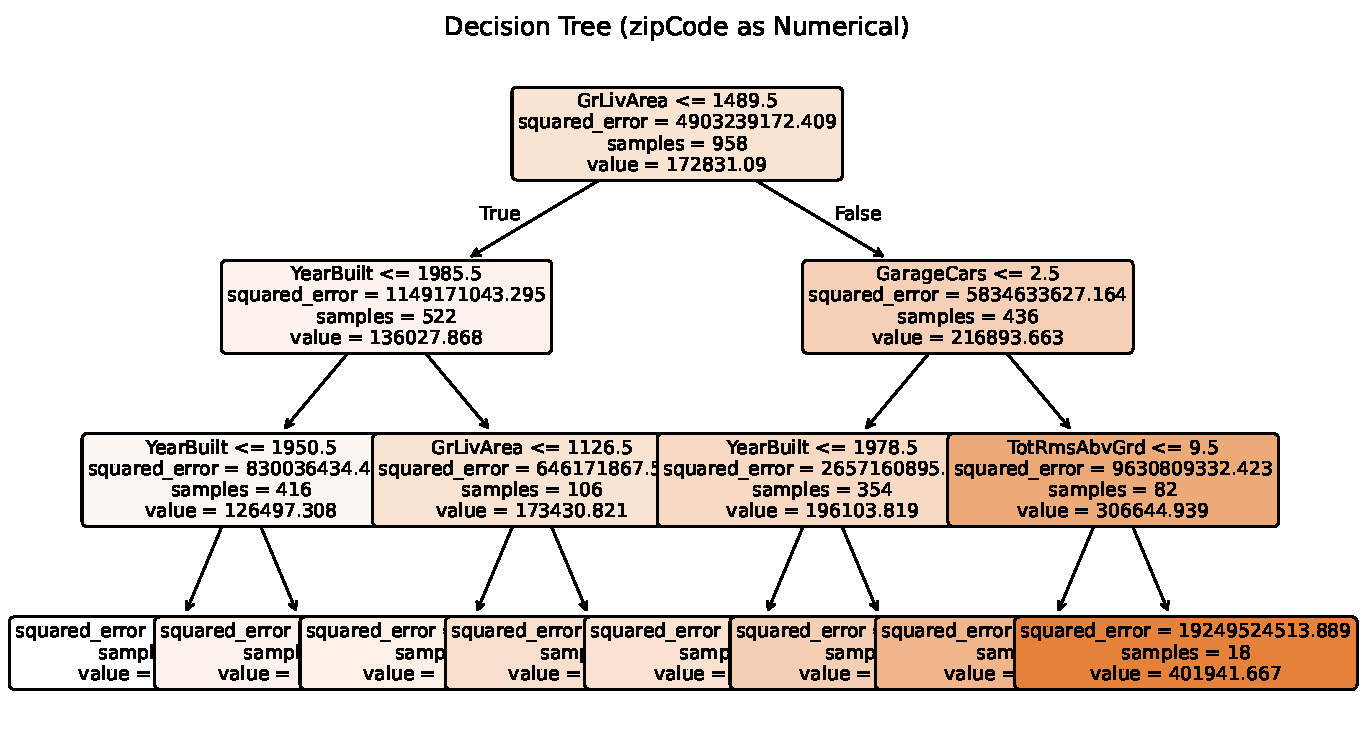
\includegraphics[keepaspectratio]{index_files/figure-pdf/cell-3-output-1.pdf}}

\subsection{Feature Importance
(Numerical)}\label{feature-importance-numerical}

\begin{longtable}[]{@{}lll@{}}
\toprule\noalign{}
& Feature & Importance \\
\midrule\noalign{}
\endhead
\bottomrule\noalign{}
\endlastfoot
2 & GrLivArea & 0.520719 \\
7 & GarageCars & 0.266960 \\
1 & YearBuilt & 0.143594 \\
6 & TotRmsAbvGrd & 0.068727 \\
0 & LotArea & 0.000000 \\
4 & HalfBath & 0.000000 \\
3 & FullBath & 0.000000 \\
5 & BedroomAbvGr & 0.000000 \\
8 & zipCode & 0.000000 \\
\end{longtable}

\subsection{Numerical Encoding Problem
(Analysis)}\label{numerical-encoding-problem-analysis}

In the numerical model, zipCode is treated as a continuous variable.
This leads to meaningless splits such as threshold comparisons between
zip codes, which do not reflect real-world relationships.

As a result, the model either underestimates or misinterprets the
importance of zipCode. Even when zipCode is important for predicting
house prices, the encoding prevents the decision tree from capturing its
true effect. This highlights how improper encoding can distort feature
importance results.

\subsection{Categorical Encoding Model (One-Hot
Encoding)}\label{categorical-encoding-model-one-hot-encoding}

\begin{longtable}[]{@{}
  >{\raggedright\arraybackslash}p{(\linewidth - 4\tabcolsep) * \real{0.3333}}
  >{\raggedright\arraybackslash}p{(\linewidth - 4\tabcolsep) * \real{0.3333}}
  >{\raggedright\arraybackslash}p{(\linewidth - 4\tabcolsep) * \real{0.3333}}@{}}
\toprule\noalign{}
\endhead
\bottomrule\noalign{}
\endlastfoot
\emph{} & \begin{minipage}[t]{\linewidth}\raggedright
\href{https://scikit-learn.org/1.8/modules/generated/sklearn.tree.DecisionTreeRegressor.html\#:~:text=criterion,-\%7B\%22squared_error\%22\%2C\%20\%22friedman_mse\%22\%2C\%20\%22absolute_error\%22\%2C\%20\%20\%20\%20\%20\%20\%20\%20\%20\%20\%20\%20\%20\%22poisson\%22\%7D\%2C\%20default\%3D\%22squared_error\%22}{criterion
{criterion: \{"squared\_error", "friedman\_mse", "absolute\_error",
"poisson"\}, default="squared\_error"\\
\strut \\
The function to measure the quality of a split. Supported criteria\\
are "squared\_error" for the mean squared error, which is equal to\\
variance reduction as feature selection criterion and minimizes the L2\\
loss using the mean of each terminal node, "friedman\_mse", which uses\\
mean squared error with Friedman\textquotesingle s improvement score for
potential\\
splits, "absolute\_error" for the mean absolute error, which minimizes\\
the L1 loss using the median of each terminal node, and "poisson"
which\\
uses reduction in the half mean Poisson deviance to find splits.\\
\strut \\
.. versionadded:: 0.18\\
Mean Absolute Error (MAE) criterion.\\
\strut \\
.. versionadded:: 0.24\\
Poisson deviance criterion.}}\strut
\end{minipage} & \textquotesingle squared\_error\textquotesingle{} \\
\emph{} & \begin{minipage}[t]{\linewidth}\raggedright
\href{https://scikit-learn.org/1.8/modules/generated/sklearn.tree.DecisionTreeRegressor.html\#:~:text=splitter,-\%7B\%22best\%22\%2C\%20\%22random\%22\%7D\%2C\%20default\%3D\%22best\%22}{splitter
{splitter: \{"best", "random"\}, default="best"\\
\strut \\
The strategy used to choose the split at each node. Supported\\
strategies are "best" to choose the best split and "random" to choose\\
the best random split.}}\strut
\end{minipage} & \textquotesingle best\textquotesingle{} \\
\emph{} & \begin{minipage}[t]{\linewidth}\raggedright
\href{https://scikit-learn.org/1.8/modules/generated/sklearn.tree.DecisionTreeRegressor.html\#:~:text=max_depth,-int\%2C\%20default\%3DNone}{max\_depth
{max\_depth: int, default=None\\
\strut \\
The maximum depth of the tree. If None, then nodes are expanded until\\
all leaves are pure or until all leaves contain less than\\
min\_samples\_split samples.\\
\strut \\
For an example of how ``max\_depth`` influences the model, see\\
:ref:`sphx\_glr\_auto\_examples\_tree\_plot\_tree\_regression.py`.}}\strut
\end{minipage} & 3 \\
\emph{} & \begin{minipage}[t]{\linewidth}\raggedright
\href{https://scikit-learn.org/1.8/modules/generated/sklearn.tree.DecisionTreeRegressor.html\#:~:text=min_samples_split,-int\%20or\%20float\%2C\%20default\%3D2}{min\_samples\_split
{min\_samples\_split: int or float, default=2\\
\strut \\
The minimum number of samples required to split an internal node:\\
\strut \\
- If int, then consider `min\_samples\_split` as the minimum number.\\
- If float, then `min\_samples\_split` is a fraction and\\
`ceil(min\_samples\_split * n\_samples)` are the minimum\\
number of samples for each split.\\
\strut \\
.. versionchanged:: 0.18\\
Added float values for fractions.}}\strut
\end{minipage} & 20 \\
\emph{} & \begin{minipage}[t]{\linewidth}\raggedright
\href{https://scikit-learn.org/1.8/modules/generated/sklearn.tree.DecisionTreeRegressor.html\#:~:text=min_samples_leaf,-int\%20or\%20float\%2C\%20default\%3D1}{min\_samples\_leaf
{min\_samples\_leaf: int or float, default=1\\
\strut \\
The minimum number of samples required to be at a leaf node.\\
A split point at any depth will only be considered if it leaves at\\
least ``min\_samples\_leaf`` training samples in each of the left and\\
right branches. This may have the effect of smoothing the model,\\
especially in regression.\\
\strut \\
- If int, then consider `min\_samples\_leaf` as the minimum number.\\
- If float, then `min\_samples\_leaf` is a fraction and\\
`ceil(min\_samples\_leaf * n\_samples)` are the minimum\\
number of samples for each node.\\
\strut \\
.. versionchanged:: 0.18\\
Added float values for fractions.}}\strut
\end{minipage} & 10 \\
\emph{} & \begin{minipage}[t]{\linewidth}\raggedright
\href{https://scikit-learn.org/1.8/modules/generated/sklearn.tree.DecisionTreeRegressor.html\#:~:text=min_weight_fraction_leaf,-float\%2C\%20default\%3D0.0}{min\_weight\_fraction\_leaf
{min\_weight\_fraction\_leaf: float, default=0.0\\
\strut \\
The minimum weighted fraction of the sum total of weights (of all\\
the input samples) required to be at a leaf node. Samples have\\
equal weight when sample\_weight is not provided.}}\strut
\end{minipage} & 0.0 \\
\emph{} & \begin{minipage}[t]{\linewidth}\raggedright
\href{https://scikit-learn.org/1.8/modules/generated/sklearn.tree.DecisionTreeRegressor.html\#:~:text=max_features,-int\%2C\%20float\%20or\%20\%7B\%22sqrt\%22\%2C\%20\%22log2\%22\%7D\%2C\%20default\%3DNone}{max\_features
{max\_features: int, float or \{"sqrt", "log2"\}, default=None\\
\strut \\
The number of features to consider when looking for the best split:\\
\strut \\
- If int, then consider `max\_features` features at each split.\\
- If float, then `max\_features` is a fraction and\\
`max(1, int(max\_features * n\_features\_in\_))` features are considered
at each\\
split.\\
- If "sqrt", then `max\_features=sqrt(n\_features)`.\\
- If "log2", then `max\_features=log2(n\_features)`.\\
- If None, then `max\_features=n\_features`.\\
\strut \\
Note: the search for a split does not stop until at least one\\
valid partition of the node samples is found, even if it requires to\\
effectively inspect more than ``max\_features`` features.}}\strut
\end{minipage} & None \\
\emph{} & \begin{minipage}[t]{\linewidth}\raggedright
\href{https://scikit-learn.org/1.8/modules/generated/sklearn.tree.DecisionTreeRegressor.html\#:~:text=random_state,-int\%2C\%20RandomState\%20instance\%20or\%20None\%2C\%20default\%3DNone}{random\_state
{random\_state: int, RandomState instance or None, default=None\\
\strut \\
Controls the randomness of the estimator. The features are always\\
randomly permuted at each split, even if ``splitter`` is set to\\
``"best"``. When ``max\_features \textless{} n\_features``, the
algorithm will\\
select ``max\_features`` at random at each split before finding the
best\\
split among them. But the best found split may vary across different\\
runs, even if ``max\_features=n\_features``. That is the case, if the\\
improvement of the criterion is identical for several splits and one\\
split has to be selected at random. To obtain a deterministic
behaviour\\
during fitting, ``random\_state`` has to be fixed to an integer.\\
See :term:`Glossary ` for details.}}\strut
\end{minipage} & 123 \\
\emph{} & \begin{minipage}[t]{\linewidth}\raggedright
\href{https://scikit-learn.org/1.8/modules/generated/sklearn.tree.DecisionTreeRegressor.html\#:~:text=max_leaf_nodes,-int\%2C\%20default\%3DNone}{max\_leaf\_nodes
{max\_leaf\_nodes: int, default=None\\
\strut \\
Grow a tree with ``max\_leaf\_nodes`` in best-first fashion.\\
Best nodes are defined as relative reduction in impurity.\\
If None then unlimited number of leaf nodes.}}\strut
\end{minipage} & None \\
\emph{} & \begin{minipage}[t]{\linewidth}\raggedright
\href{https://scikit-learn.org/1.8/modules/generated/sklearn.tree.DecisionTreeRegressor.html\#:~:text=min_impurity_decrease,-float\%2C\%20default\%3D0.0}{min\_impurity\_decrease
{min\_impurity\_decrease: float, default=0.0\\
\strut \\
A node will be split if this split induces a decrease of the impurity\\
greater than or equal to this value.\\
\strut \\
The weighted impurity decrease equation is the following::\\
\strut \\
N\_t / N * (impurity - N\_t\_R / N\_t * right\_impurity\\
- N\_t\_L / N\_t * left\_impurity)\\
\strut \\
where ``N`` is the total number of samples, ``N\_t`` is the number of\\
samples at the current node, ``N\_t\_L`` is the number of samples in
the\\
left child, and ``N\_t\_R`` is the number of samples in the right
child.\\
\strut \\
``N``, ``N\_t``, ``N\_t\_R`` and ``N\_t\_L`` all refer to the weighted
sum,\\
if ``sample\_weight`` is passed.\\
\strut \\
.. versionadded:: 0.19}}\strut
\end{minipage} & 0.0 \\
\emph{} & \begin{minipage}[t]{\linewidth}\raggedright
\href{https://scikit-learn.org/1.8/modules/generated/sklearn.tree.DecisionTreeRegressor.html\#:~:text=ccp_alpha,-non-negative\%20float\%2C\%20default\%3D0.0}{ccp\_alpha
{ccp\_alpha: non-negative float, default=0.0\\
\strut \\
Complexity parameter used for Minimal Cost-Complexity Pruning. The\\
subtree with the largest cost complexity that is smaller than\\
``ccp\_alpha`` will be chosen. By default, no pruning is performed.
See\\
:ref:`minimal\_cost\_complexity\_pruning` for details. See\\
:ref:`sphx\_glr\_auto\_examples\_tree\_plot\_cost\_complexity\_pruning.py`\\
for an example of such pruning.\\
\strut \\
.. versionadded:: 0.22}}\strut
\end{minipage} & 0.0 \\
\emph{} & \begin{minipage}[t]{\linewidth}\raggedright
\href{https://scikit-learn.org/1.8/modules/generated/sklearn.tree.DecisionTreeRegressor.html\#:~:text=monotonic_cst,-array-like\%20of\%20int\%20of\%20shape\%20\%28n_features\%29\%2C\%20default\%3DNone}{monotonic\_cst
{monotonic\_cst: array-like of int of shape (n\_features),
default=None\\
\strut \\
Indicates the monotonicity constraint to enforce on each feature.\\
- 1: monotonic increase\\
- 0: no constraint\\
- -1: monotonic decrease\\
\strut \\
If monotonic\_cst is None, no constraints are applied.\\
\strut \\
Monotonicity constraints are not supported for:\\
- multioutput regressions (i.e. when `n\_outputs\_ \textgreater{} 1`),\\
- regressions trained on data with missing values.\\
\strut \\
Read more in the :ref:`User Guide `.\\
\strut \\
.. versionadded:: 1.4}}\strut
\end{minipage} & None \\
\end{longtable}

\subsection{Tree Visualization
(Categorical)}\label{tree-visualization-categorical}

\pandocbounded{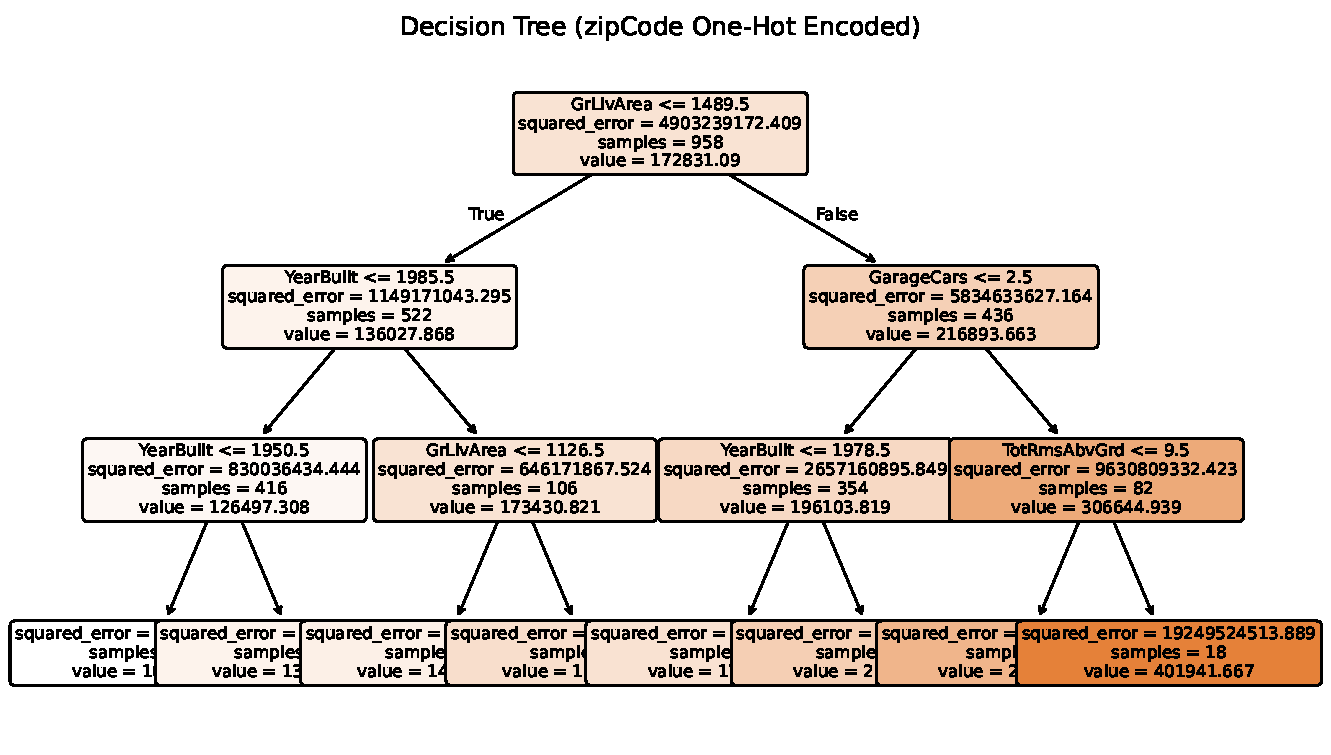
\includegraphics[keepaspectratio]{index_files/figure-pdf/cell-6-output-1.pdf}}

\subsection{Feature Importance
(Categorical)}\label{feature-importance-categorical}

\begin{longtable}[]{@{}lll@{}}
\toprule\noalign{}
& Feature & Importance \\
\midrule\noalign{}
\endhead
\bottomrule\noalign{}
\endlastfoot
2 & GrLivArea & 0.520719 \\
7 & GarageCars & 0.266960 \\
1 & YearBuilt & 0.143594 \\
6 & TotRmsAbvGrd & 0.068727 \\
0 & LotArea & 0.000000 \\
4 & HalfBath & 0.000000 \\
3 & FullBath & 0.000000 \\
5 & BedroomAbvGr & 0.000000 \\
8 & zipCode\_50010 & 0.000000 \\
9 & zipCode\_50011 & 0.000000 \\
10 & zipCode\_50012 & 0.000000 \\
11 & zipCode\_50013 & 0.000000 \\
12 & zipCode\_50014 & 0.000000 \\
13 & zipCode\_50015 & 0.000000 \\
14 & zipCode\_50016 & 0.000000 \\
15 & zipCode\_50017 & 0.000000 \\
16 & zipCode\_50018 & 0.000000 \\
17 & zipCode\_50019 & 0.000000 \\
18 & zipCode\_50020 & 0.000000 \\
19 & zipCode\_50021 & 0.000000 \\
20 & zipCode\_50022 & 0.000000 \\
21 & zipCode\_50023 & 0.000000 \\
22 & zipCode\_50024 & 0.000000 \\
23 & zipCode\_50025 & 0.000000 \\
24 & zipCode\_50026 & 0.000000 \\
25 & zipCode\_50027 & 0.000000 \\
26 & zipCode\_50028 & 0.000000 \\
27 & zipCode\_50029 & 0.000000 \\
28 & zipCode\_50030 & 0.000000 \\
29 & zipCode\_50031 & 0.000000 \\
30 & zipCode\_50032 & 0.000000 \\
31 & zipCode\_50033 & 0.000000 \\
32 & zipCode\_50034 & 0.000000 \\
\end{longtable}

\subsection{One-Hot Encoding Solution
(Analysis)}\label{one-hot-encoding-solution-analysis}

When zipCode is one-hot encoded, the model can evaluate each geographic
area independently. This allows the decision tree to identify specific
zip codes that have a strong relationship with housing prices.

Unlike numerical encoding, this approach preserves the categorical
nature of the variable and results in more meaningful splits. It
improves interpretability and ensures that location effects are
correctly captured in feature importance.

\subsection{Discussion}\label{discussion}

\begin{enumerate}
\def\labelenumi{\arabic{enumi}.}
\tightlist
\item
  \textbf{Numerical vs Categorical Analysis:}
\end{enumerate}

Zip code should be modeled as a categorical variable, specifically a
non-ordinal categorical variable. There is no meaningful ranking or
numeric relationship between zip codes, so treating them as numbers
introduces false assumptions.

When encoded numerically, the decision tree imposes artificial order and
evaluates meaningless thresholds. This leads to incorrect feature
importance results, where an important variable may appear irrelevant.
Proper categorical encoding allows the model to recognize differences
between locations without imposing structure that does not exist.

\begin{enumerate}
\def\labelenumi{\arabic{enumi}.}
\setcounter{enumi}{1}
\tightlist
\item
  \textbf{R vs Python Implementation Analysis:}
\end{enumerate}

A key limitation of :contentReference{oaicite:0} is that it does not
natively support categorical variables in decision trees. Instead, all
inputs must be numerical, which forces users to encode categories
manually.

According to the documentation: \textgreater{} ``Decision trees in
scikit-learn do not support categorical variables directly.''

This restriction means the model can only split on numerical thresholds,
not on groups or subsets of categories. In contrast, R-based
implementations (such as \texttt{rpart}) can directly handle categorical
variables and split them into meaningful subsets.

As a result, R provides more natural and interpretable modeling for
categorical data, while Python requires workarounds like one-hot
encoding, which can still limit how relationships are captured.

\begin{enumerate}
\def\labelenumi{\arabic{enumi}.}
\setcounter{enumi}{2}
\tightlist
\item
  \textbf{Alternative Python Approaches}
\end{enumerate}

Some advanced Python libraries, such as CatBoost, can handle categorical
variables directly without one-hot encoding. These models can split on
subsets of categories rather than numeric thresholds.

Using such approaches, a model could group multiple zip codes together
in a single split, capturing more complex relationships between location
and price. This more closely reflects real-world patterns, where
neighborhoods may share similar characteristics.

However, these methods are more complex and require additional setup.
For most standard workflows, one-hot encoding remains the practical
solution, even though it has limitations compared to true
categorical-aware models.

\subsection{Conclusion}\label{conclusion}

This analysis highlights that decision trees are only as interpretable
as the data preparation behind them. Treating categorical variables as
numerical can completely hide meaningful relationships and lead to
incorrect conclusions about feature importance.

Proper encoding is not just a technical detail---it is essential for
ensuring that model insights reflect reality. In this case, correcting
the encoding of zipCode transformed it from an ignored variable into a
meaningful predictor, reinforcing the importance of thoughtful data
preprocessing in machine learning.




\end{document}
